% Sandia National Laboratories is a multimission laboratory managed and
% operated by National Technology & Engineering Solutions of Sandia, LLC, a
% wholly owned subsidiary of Honeywell International Inc., for the U.S.
% Department of Energy’s National Nuclear Security Administration under
% contract DE-NA0003525.

% Copyright 2002-2021 National Technology & Engineering Solutions of Sandia,
% LLC (NTESS).


\begin{Device}\label{T_DEVICE}

\symbol
{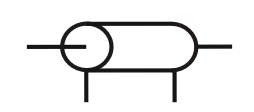
\includegraphics{translineSymbol}}

\device
\begin{alltt}
T<name> <port 1 (+) node> <port 1 (-) node>
+ <port 2 (+) node> <port 2 (-) node>
+ Z0=<value> [TD=<value>] [F=<value> [NL=<value>]]
\end{alltt}

\examples
\begin{alltt}
Tline inp inn outp outn Z0=50 TD=1us
Tline2 inp inn outp outn Z0=50 F=1meg NL=1.0
\end{alltt}

\comments

The lossless transmission line device is a two port (\texttt{A} and
\texttt{B}), bi-directional delay line. The \texttt{(+)} and
\texttt{(-)} nodes define the polarity of a positive voltage at a port.

\texttt{Z0} is the characteristic impedance. For user convenience, 
\texttt{ZO} (``Zee Oh'') is an allowed synonym for \texttt{Z0} (``Zee Zero'').

The transmission line's length is specified by either \texttt{TD} (a delay in
seconds) or by the combination of \texttt{F} and \texttt{NL} (a frequency in Hz and 
the relative wavelength at \texttt{F}). \texttt{NL} defaults to 0.25 (\texttt{F} is 
the quarter-wave frequency).  If \texttt{F} is given, the time delay is 
computed as $\frac{NL}{F}$.  

While both \texttt{TD} and \texttt{F} are optional, at least one of them must be given.
It is an instance line error if both are given.

Lead currents for the two terminals (1 and 2) of the lossless transmission device 
(e.g.,for the T device \texttt{line2}) are accessed via \texttt{I1(Tline2)} and 
\texttt{I2(Tline2)}.  The polarity conventions are that positive current flows into
the positive node of the specified terminal, and negative current flows out of the
positive node of the specified terminal.

Power for the lossless transmission line is calculated as $I_1 \cdot \Delta V_1 + 
I_2 \cdot \Delta V_2$, where the voltage drops ($\Delta V_1$ and $\Delta V_2$) are the 
voltage drops between the positive and negative terminals of each port (e.g., 
$\Delta V = (V_+ - V_-)$).  The sign conventions for the lead currents $I_1$ and $I_2$ 
were given in the previous paragraph.  This definition can be viewed as the instantaneous
sum of the power flowing into terminal 1 and the power flowing into terminal 2.
This definition for power for the lossless transmission line may differ from 
commercial simulators, such as HSPICE.  

The lossless transmission line device does not work with AC analysis
at this time.  Lossless transmission line models will need to be
replaced with lumped transmission line models (YTRANSLINE) when used
in AC analysis.  The lossless transmission line does work correctly in
harmonic balance simulation.

\end{Device}

\paragraph{Instance Parameters}
% This table was generated by Xyce:
%   Xyce -doc T 1
%
\index{ideal transmission line!device instance parameters}
\begin{DeviceParamTableGenerated}{Ideal Transmission Line Device Instance Parameters}{T_1_Device_Instance_Params}
F & Frequency & Hz & 0 \\ \hline
NL & Length in wavelengths & -- & 0.25 \\ \hline
TD & Time delay & s & 0 \\ \hline
Z0 & Characteristic Impedance & $\mathsf{\Omega}$ & 0 \\ \hline
ZO & Characteristic Impedance & $\mathsf{\Omega}$ & 0 \\ \hline
\end{DeviceParamTableGenerated}

